\documentclass[../setup.tex]{subfiles}
\graphicspath{{../images}}

\begin{document}

\title{Notes from How to Prove It}
\author{Julian Dominic}
\date{28 July 2022}
\pagenumbering{gobble}
\maketitle
\clearpage


% ===== Define a preface environment =====
\newcommand{\prefacename}{Preface}
\newenvironment{preface}{
    {\noindent \bfseries \Huge \prefacename}
    \begin{center}
        % \phantomsection \addcontentsline{toc}{chapter}{\prefacename} % enable this if you want to put the preface in the table of contents
        \thispagestyle{plain}
    \end{center}%
}



\preface
I wrote these notes principally FOR understanding, they are meant for future reference for a refresher on what I have learnt. As such, certain definitions may not be exactly precise but are rephrased into simpler terms. \\
I am using the first edition of the book. ISBN 0-521-44663-5 \\
Honestly, I don't have much to say, I just thought that a preface would be cool. Let's start our journey now.



\tableofcontents
\pagenumbering{gobble}
\clearpage

\pagenumbering{arabic}
\setcounter{page}{1}



\section{Sentential Logic}
\subsection{Deductive reasoning and logical connectives}
In an \textit{argument}, we arrive at \textbf{valid} \textit{conclusions} assuming that the \textit{premises} are \textbf{true}. \\ 
Premises and conclusion are often referred to as conditions and outcomes respectively. \\
If all the premises are \textbf{true}, then the conclusion should be \textbf{true}. However, for the case where the conclusion is \textbf{false} while the premises are \textbf{true}, the argument is \textbf{invalid}.

\subsubsection{Logical Operators}
{
\centering
\begin{tabular}{| c | c | c |}
\hline
Symbol & Meaning & Description \\
\hline
& & \\
$\lor$ & OR & Disjunction \\
& & \\
$\land$ & AND & Conjunction \\
& & \\
$\lnot$ & NOT & Negation \\
& & \\
\hline
\end{tabular} \\
}



\subsection{Truth tables}
A truth table must be able to represent all possible combinations of the variables, premises and conclusions.\\
\\

{
\centering
% I couldn't get the three tables to be side-by-side and centered properly so here comes minipages and manual spaces
\ \ \ \ \ \ \ \ \ \ \ \ \ \ \ \ \ \ \ \ \ \ \
\begin{minipage}[t]{0.32\textwidth}
	\begin{tabular}[t]{|c|c|c|}
		\hline
		$P$&$Q$&$P\lor Q$ \\
		\hline
		F&F&F \\
		F&T&T \\
		T&F&T \\
		T&T&T \\
		\hline
	\end{tabular}
\end{minipage}
\quad
\begin{minipage}[t]{0.32\textwidth}
	\begin{tabular}[t]{|c|c|c|}
		\hline
		$P$&$Q$&$P\land Q$ \\
		\hline
		F&F&F \\
		F&T&F \\
		T&F&F \\
		T&T&T \\
		\hline
	\end{tabular} 
\end{minipage}
\quad
\begin{minipage}[t]{0.32\textwidth}
	\begin{tabular}[t]{|c|c|}
		\hline
		$P$&$\lnot P$ \\
		\hline
		F&T \\
		T&F \\
		\hline
	\end{tabular}
\end{minipage}
}
\\ 
\\
In this case, we see that our variables (or statements), $P$ and $Q$ have their individual column to assign a value -- \textbf{True} or \textbf{False} -- to them. \\
We use our logical operators to make a new statement from $P$ and $Q$ which can be $P\land Q$, and assign a value to the new statement. \\
\\
It is important note that the number of variables will dictate the number of rows that the truth table will have. Construct a truth table for the following set of variables, $\{P\}$, $\{P, Q\}$, $\{P, Q, R\}$. \\
The pattern that we find is that as the number of variables increases, the number of rows increases two-fold. \\
\[ \text{Number of Rows} = 2^{\text{Number of Variables}} \]
\\
There are some special truth tables where the column for the conclusion always has the same value (either all \textit{true} or all \textit{false}) for every combination of the variables' values. \\
\\
When the conclusion is always \textit{true}, we say that the conclusion's statement is a \textbf{tautology}. Construct a truth table for $P\lor\lnot P$.\\
Similarly, when the conclusion is always \textit{false}, we say that the conclusion's statement is a \textbf{contradiction}. Construct a truth table for $P \land\lnot P$. \\

\begin{remark}
\textit{Tautologies} and \textit{Contradictions} are not the only laws that govern logic. Do see the logic document for more.
\end{remark}



\subsection{Variables and sets}
\subsubsection{Sets}
A set is a collection of elements. The order of the elements in the set does not matter. If an element appears more than once, it is still the same set. \\
\[ \{3, 7, 14\} \equiv \{7, 3, 14\} \equiv \{14, 3, 7, 7\} \]
\\
When the set is infinite or has too many elemnts to list, we will define it explicitly. Suppose we have the following set $P$. \\

\[ P = \{x \ |\  x \text{ is a prime number}\} \]
\\
How we read $P = \{x | x \text{is a prime number}\}$ is ``$P$ is equal to the set of all $x$ such that $x$ is a prime number.'' Which also means that $P$ contains all values of $x$ that make the statement ``$x$ is a prime number'' true. \\
Some direct translations of the symbols into words would be (i) ``\{\}'' means ``the set of'', and (ii) ``$|$'' means ``such that''. \\
\\
Sets like $P$ have an \textbf{elementhood test} for the set; in this case, the \textit{elementhood test} is being a prime number. Any value of $x$ that makes the statement come out true, passes the test and is an element of the set. \\
\begin{theorem}[Truth Set]
The \textbf{Truth set} of a statement $P(x)$ is the set of all values of $x$ that make the statement $P(x)$ true. In other words, it is the set defined by using the statement $P(x)$ as the elementhood test: \\
\[ \text{Truth set of } P(x) = \{x \ | \ P(x)\} \]
\end{theorem}

\subsubsection{Understanding variables used in sets}
There are two types of variables that can appear in a set; \textbf{Free variables} and \textbf{Bound variables}. \textit{Free variables} are variables that will make the statement either \textit{True} or \textit{False} while \textit{Bound variables} are variables whose values we do not need to know (they can be considered \textit{dummy variables}). Lets consider the following example, \\
\\
 \[ y \in \{x \ | \ x^2 < 9\} \] 
\\
For any number $y$, to verify $y \in \{x \ | \ x^2 < 9\}$, we have to check $y^2 < 9$. Since $y \in \{x \ | \ x^2 < 9\}$ is just a roundabout way of saying $y^2 < 9$, it follows that we do not need to care about the value of $x$. Rather, only the value of $y$ is required. Thus, we can say that $y$ is a \textit{free variable} while $x$ is a \textit{bound variable}. As such, we can go further and replace $x$ with any other variable except $y$ because we do not need to care what $x$ is. As such, it can even be $y \in \{w\ | \ w^2 < 9\}$ where $y$ is \textit{free} and $w$ is \textit{bound}. Notice that $x^2 < 9$ makes $x$ a \textit{free variable}. We can say that that statement $P(x)$ in $\{x \ | \ P(x)\}$ \textbf{binds} the variable $x$. 


\begin{remark}
In general, the statement $y \in \{x\ |\ P(x)\} \Rightarrow P(y)$ and $y \notin \{x\ |\ P(x)\} \Rightarrow \lnot P(y)$. \\
It is also important to note that ${x\ |\ P(x)}$ is not a statement. It is a set because of the curly brackets ``\{\}''
\end{remark}

\begin{theorem}[Universe of Discourse]
The \textbf{Universe of Discourse}, $U$, is the set of all possible values for the variables. We can say things such as $\{x \in U\ |\ P(x)\}$: The set of all $x$ in $U$ such that $P(x)$. For a set that has the \textit{universe of discourse} defined, an element of the set has to pass two tests, $x \in U$ and $P(x)$. Therefore, in general, $y \in \{x\in A\ |\ P(x)\} \Rightarrow y\in A \land P(y)$. \\
If $P(x)$ is false for every possible value of $x$, it yields a truth set with no elements. As such, we get the \textbf{empty set}/\textbf{null set}; $\emptyset$ or $\{\}$ where the contents inside the curly brackets are blank. For example, \\
\[\{x\in\mathbb{Z} \ |\ x \neq x\} = \emptyset = \{\}\]
\end{theorem}

\begin{remark}
$\emptyset \neq \{\emptyset\}$. $\emptyset$ is a set while $\{\emptyset\}$ is a set of a set.
\end{remark}



\subsection{Operations on two sets}
\begin{theorem}[Intersection of sets]
The \textbf{Intersection} of sets -- as the name suggests -- will yield the set that contains elements that exists in both of the sets. Simply, it contains elements that the sets have in common.
\[A\cap B = \{x\ |\ x\in A\ \text{and } x\in B \}\]
\begin{figure}[H]
    \centering
    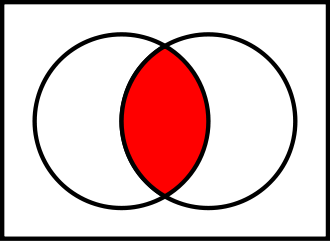
\includegraphics[scale=0.6]{Venn Diagram-Intersection.png}
    \caption{Source from Wikipedia}
\end{figure}
\end{theorem}

\begin{theorem}[Disjoint]
$A$ and $B$ are \textbf{disjoint} if they have no elements in common; the \textbf{intersection} of the sets $A$ and $B$ does not exist -- the set is empty. This is also known as \textbf{mutually exclusive}. Therefore, we can say that $A$ and $B$ are \textit{mutually exclusive}.
\[A\cap B = \emptyset\]
\begin{figure}[H]
    \centering
    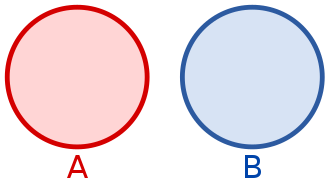
\includegraphics[scale=0.6]{Venn Diagram-Disjoint.png}
    \caption{Source from Wikipedia}
\end{figure}
\end{theorem}


\begin{theorem}[Union of two sets]
The \textbf{Union} of sets will yield the set that contains elements that come from any and all of the sets. Essentially, it is the amalgamation of all the elements from every set. It is important to note that in Mathematics, the word \textbf{or} is used `inclusively'; Consider the example below, we want to get elements that are in either $A$ or $B$ or both. While in conversation, we may think of \textbf{or} as an exclusive term such as when making a decision between two choices.
\[A\cup B = \{x\ |\ x\in A\ \text{or } x\in B \}\]
\begin{figure}[H]
    \centering
    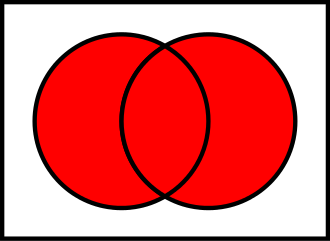
\includegraphics[scale=0.6]{Venn Diagram-Union.png}
    \caption{Source from Wikipedia}
\end{figure}
\end{theorem}



\begin{theorem}[Difference of two sets]
The \textbf{Difference} of sets will yield the set that contains elements that are \textit{exclusive} to set $A$. \text{Exclusive} is being used in its literal meaning here; we do not include an element that can be found in more than one set, the element has to be unique.   
\[A\setminus B = \{x\ |\ x\in A\ \text{and } x\notin B \}\]
\begin{figure}[H]
    \centering
    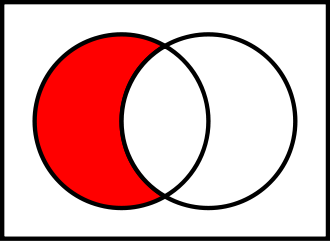
\includegraphics[scale=0.6]{Venn Diagram-Difference.png}
    \caption{Source from Wikipedia}
\end{figure}
\end{theorem}


\begin{theorem}[Symmetric Difference of two sets]
The \textbf{Symmetric Difference} of sets will yield the set that contains elements that are in either $A$ or $B$ but not both. To put it plainly, it is the set that contains elements that are exclusive to both $A$ and $B$. You can think of it as the \textbf{union} of $A$ and $B$ without their \textbf{intersection}.
\[A \triangle B = (A\setminus B) \cup (B\setminus A)\]
\begin{figure}[H]
    \centering
    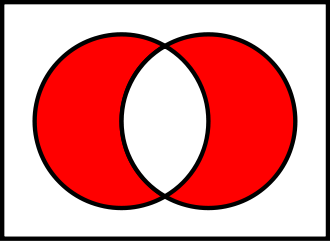
\includegraphics[scale=0.6]{Venn Diagram-SymmetricDifference.png}
    \caption{Source from Wikipedia}
\end{figure}
\end{theorem}

\begin{theorem}[Subset]
$A$ is a \textbf{subset} of $B$ if every element of $A$ is also an element of $B$. It is really just saying that $B$ is the `bigger brother' that contains $A$ . There are also \textbf{proper subsets} where $A$ is a subset of $B$ but not equal to $B$ ($A$ cannot have every single element that $B$ has).
\begin{align*}
A &\subseteq B \text{\ \ \ \ (Subset)} \\
A &\subset B \text{\ \ \ \ (Proper Subset)}
\end{align*}
\begin{figure}[H]
    \centering
    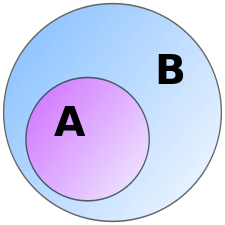
\includegraphics[scale=0.6]{Venn Diagram-ProperSubset.png}
    \caption{Source from Wikipedia}
\end{figure}
\end{theorem}

\subsection{The conditional and biconditional connectives}
\subsubsection{Conditional Statement}
\begin{theorem}[Conditional Statement]
 \textbf{Conditional statements} introduces a new logical connective, $\rightarrow$. With reference to the expression below, $P\rightarrow Q$ is read as `\textbf{If} $P$ \textbf{then} $Q$'. $P$ and $Q$ are known as the \textit{antecedent} and \textit{consequent} respectively.
\[P\rightarrow Q\ = \lnot P \lor Q \]
\end{theorem}



\begin{center}
	\begin{tabular}[t]{| c | c | c |}
		\hline
		$P$ & $Q$ & $P\rightarrow Q$ \\
		\hline
		F & F & T \\
		F & T & T \\
		T & F & F \\ 
		T & T & T \\
		\hline
	\end{tabular}
\end{center}
\phantom \\ \\
While using the equivalent formula $P\rightarrow Q\ =\ \lnot P \lor Q$ is easier to calculate the values for the truth table, lets find the motivation to fill it in just by thinking about \textbf{if} and \textbf{then}. \\
\\
The last row is painfully obvious. \textbf{If} $P$ is \textit{true} \textbf{then} $Q$ is clearly \textit{true}. \\
The third row is a little tricky but quite straightforward. There is no possible case for $P$ to be \textit{true} and $Q$ to be \textit{false} because \textbf{if} $P$ is \textit{true} \textbf{then} $Q$ \textit{must} be \textit{true}. Therefore, the statement is \textit{false}. \\
For the remaining rows, lets use an example to justify our answers. Let $P$ stand for the statement that $x > 2$, and $Q$ stand for the statement that $x^2 > 4$. For the first row, consider $x = 1$, it follows that $x^2 = 1 < 4$. I did not mention anything about an $x$-value that is less than or equal to 2; As such, it does not invalidate my claim that `\textbf{If} $x > 2$ \textbf{then} $x^2 > 4$'. Therefore, the statement is \textit{true}. Finally, for the second row, consider $x = -5$, it follows that $x^2 = 25 > 4$. Note, in a similar fashion for my justification for the first row, I still have not said anything that would invalidate my statement that earlier. Thus, the statement is \textit{true}. 

\begin{remark}
One may question why not we just claim that $P\rightarrow Q$ is false for the first two rows? In our reasoning, we just said that our variables did not invalidate our statement so the `truth'-value of our statement is actually unknown. \\ To quote: ``We accept a basic axiom of logic that tell us that every statement is either true or false, so we have to pick one. In mathematics, we find it more useful to take it to be true, but this is not necessary (for all).'' 
\end{remark}
\phantom \\ \\
The \textbf{Converse} of any \textit{conditional statement} is going in the opposite direction of its particular \textit{conditional statement}. The thought process of considering the \textbf{converse} is \textit{if} $P$ \textit{then} $Q$, but \textit{if} $Q$ \textit{then} $P \equiv \boldsymbol{Q \rightarrow P}$?\\
\\
The \textbf{Contrapositive} of any \textit{conditional statement} is going in the opposite direction of its particular \textit{conditional statement} \textbf{and} \textit{negating} the variables. More often than not, it is often confused with the \textit{converse}. This is because people often confuse the thought process of considering the \textbf{contrapositive} which would be seeing that $P \rightarrow Q \equiv \lnot P\lor Q \equiv Q \lor\lnot P \equiv \boldsymbol{\lnot Q \rightarrow \lnot P}$. One way to think about it is to break `\textbf{contrapositive}' into `\textit{contra}' and `\textit{positive}', as such, there should be no positive terms. Hence, there are negations on the variables.

\begin{theorem}[Biconditional Statement]
$P \rightarrow Q$ and $Q \rightarrow P$ are not equivalent but more often than not, we want to say that both are true. This where \textbf{Biconditional statements} come in. We want to fufill two conditions at once (which is why it is called \textbf{biconditional}). \\
With reference to the example below, $P \longleftrightarrow Q$ can be read as mainly read as `$P$ \textbf{if and only if} $Q$' (some replace \textit{if and only if} by \textit{iff} for simplicity). It is read this way because of the way the \textbf{conditional} statements are formed which is  $Q \rightarrow P$ is read as `$P$ if $Q$' and $P \rightarrow Q$ is read as `$P$ only if $Q$'.
% \longleftrightarrow -- \leftrightarrow both work. I prefer the former.
\[ \boldsymbol{P \longleftrightarrow Q} \equiv (P \rightarrow Q) \land (Q \rightarrow P) \equiv (P \rightarrow Q) \land (\lnot P \rightarrow \lnot Q)\]
\end{theorem}

\begin{remark}
There are several other ways to which the \textbf{conditional} and \textbf{biconditional} statements can be read. \\
$P \rightarrow Q$:
\begin{itemize}
	\item If $P$ then $Q$.
	\item $P$ implies $Q$.
	\item $Q$, if $P$.
	\item $P$ only if $Q$.
	\item $P$ is a sufficient condition for $Q$.
	\item $Q$ is a necessary condition for $P$.
\end{itemize} 
$P \longleftrightarrow Q$:
\begin{itemize}
	\item $P$ if and only if $Q$ or $P$ iff $Q$.
	\item $P$ is a necessary and sufficient condition for $Q$.
\end{itemize}
\end{remark}



\section{Quantificational Logic}
\subsection{Quantifiers}
\begin{theorem}[Universal Quantifier]
To say that $P(x)$ is \textbf{true} for \textbf{every} value of $x$ in the universe of discourse $U$, $P(x)$ is universally \textbf{true}.
\[\forall xP(x): \text{For all } x, P(x).\]
\end{theorem}

\begin{theorem}[Existential Quantifier]
To say that $P(x)$ is \textbf{true} for \textbf{at least one} value of $x$ in the universe of discourse $U$.
\[\exists xP(x): \text{There exists an $x$ such that $P(x)$}\] 

To say that there is exactly one value of $x$ in the universe of discourse $U$, such that $P(x)$.
\[\exists !xP(x) \equiv \exists x\left[P(x)\land \lnot\exists y\left(P(y)\land y\neq x\right)\right]\]
\end{theorem}


\subsection{Equivalences involving quantifiers}
\begin{itemize}
	\item $\lnot\forall xP(x) \equiv \exists x\lnot P(x)$
	\item $\lnot\exists xP(x) \equiv \forall x\lnot P(x)$
	\item $\{x\in U \mid P(x)\} \equiv \{x \mid P(x)\}$
	\item $\exists x \in A \ P(x) \equiv \exists x \left(x\in A \land P(x)\right)$
	\item $\forall x \in A \ P(x) \equiv \forall x \left(x\in A \rightarrow P(x)\right)$
	\item $A\subseteq B \equiv \forall x(x\in A \rightarrow B) \equiv \forall x\in A (x\in B)$
	\item $\forall x\left(P(x) \land Q(x)\right) \equiv \forall xP(x) \land \forall xQ(x)$
	\item $\forall x\left(P(x) \lor Q(x)\right) \not\equiv \forall xP(x) \lor \forall xQ(x)$
	\item $\exists x\left(P(x) \land Q(x)\right) \not\equiv \exists xP(x) \land \exists xQ(x)$
	\item $\exists x\left(P(x) \lor Q(x)\right) \equiv \exists xP(x) \lor \exists xQ(x)$
\end{itemize}
\phantom \\
Consider the statement, ``Nobody is perfect'', and express it in a logical form. It is often incorrectly written as $\lnot\forall xP(x)$ where $x$ is a person, and $P(x)$ is the statement that $x$ is perfect. $\lnot\forall xP(x)$ is saying that `Not everybody is perfect.' which implies that there is at least one person that is not perfect (see the first item in the list above). When we see $\lnot\forall x$, we immediately think of the complement of everyone which is none. However, that is wrong; `Not' everyone is actually `someone'. Therefore, the answer should be $\forall x\lnot P(x)$ or $\lnot\exists xP(x)$ where they mean `Everyone is not perfect' and `There is not a single person who is perfect' respectively. \\

\clearpage
\phantom \\ \\
Consider the following, if $A = \emptyset = \{\}$, $\forall x \in A \ P(x)$ is vacuously true (there isn't a value of $x$ for which $x \in A$ is true) and $\lnot\forall x \in A \ P(x)$ is false. \\
\begin{align*}
\lnot\forall x \in A \ P(x) &\equiv \lnot\forall x(x\in A \rightarrow P(x)) \\
&\equiv \lnot\forall x(x \notin A \lor P(x)) \\ 
&\equiv \exists x(x \in A \land \lnot P(x)) \\
&\equiv \exists x\in A \ \lnot P(x)
\end{align*}
$\exists x\in A \ \lnot P(x)$ says that `There exists at least one value of $x$ st. $\lnot P(x)$'. However, since  $A = \emptyset = \{\}$, there is no such value of $x$ and therefore, the statement is false.


\begin{remark}
Changing the order of the quantifiers do not matter if they are the same type.
\begin{itemize}
	\item $\forall x\forall y \equiv \forall y\forall x$
	\item $\exists x\exists y \equiv \exists y\exists x$
\end{itemize}
It is also important to note that $\forall x \in A$ and $\exists x \in A$ are bounded quantifiers. Consider $\forall x \in U \ (x\geq 0)$ where $U$ can be $\mathbb{R}$ or $\mathbb{N}$.
\end{remark}


\subsection{More operations on sets}
Consider the following, 
\begin{itemize}
	\item $S = \{x \mid \exists n \in \mathbb{N} \ (x = n^2)\} = \{n^2 \mid n \in \mathbb{N}\}$
	\item $x \in \{n^2 \mid n \in \mathbb{N}\} \ equiv \exists n \in \mathbb{N} \ (x = n^2)$
\end{itemize}
Suppose $P = \{p_1, p_2, p_3, \dots, p_100\}$, and we can represent the elements as $p_i$ where $i \in I$. $I = \{1, 2, 3, \dots, 100\} = \{i \in \mathbb{N} \mid 1 \leq i \leq 100\}$. Therefore, $P = \{p_i \mid i \in I\}$ \\
$I$ is called the \textbf{index set} because $i$ is the \textbf{index}, and $\{p_i \mid i \in I\}$ is called an \textbf{indexed family}. \\
\\
In general, Indexed Family: $A = \{x_i \mid i \in I\} = \{x \mid \exists i \in I \ (x = x_i)\} \Rightarrow x \in \{x_i \mid i \in I\} \equiv \exists i \in I \ (x = x_i)$ 

\begin{example}[How to Prove It 2.3.1]
\phantom \\
\begin{enumerate}
	\item $y \in \{\sqrt[3]{x} \mid x \in \mathbb{Q}\} \equiv \exists x \in \mathbb{Q} \ (y=\sqrt[3]{x})$
	\item $\{x_i \mid i \in I\} \subseteq A \Rightarrow x \in \{x_i \mid i \in I\} \subseteq A \equiv \forall x\left[\exists i \in I \ (x = x_i) \rightarrow x \in A \right] \equiv \forall i \in I \ (x_i \in A)$
\end{enumerate}
\end{example}

\clearpage

\begin{theorem}[Families of sets]
$\mathcal{F}$: Families of sets where $\mathcal{F}$ is a set of other sets. For example, $\mathcal{F}$ = $\{A, B, C\}$ where $A$, $B$, $C$ are sets.
\end{theorem}

\begin{theorem}[Power Set]
Suppose $A$ is a set. The \textbf{Power Set} of $A$ is dentoed by $\mathcal{P}(A)$. $\mathcal{P}(A)$ is the set whose elements are all the subsets of $A$. \\
\[\mathcal{P}(A) = \{x \mid x \subseteq A\}\]
where $x$ is a set. \\
For example, $A = \{7, 12\} \Rightarrow \mathcal{P}(A) = \{\emptyset, \{7\}, \{12\}, \{7, 12\}\}$ \\
$\mathcal{P}(\emptyset) = \{\emptyset\}$
\end{theorem}
\begin{remark}
The empty set, $\emptyset$, is always a subset of every set including iteself, $\emptyset$. 
\end{remark}

\begin{example}[How to Prove It 2.3.3]
\phantom \\
\begin{enumerate}
	\item $x \in \mathcal{P}(A)$ means that $x$ is a subset of $A$. \\
		$\Rightarrow x \subseteq A \equiv \forall y (y \in x \rightarrow y \in A)$
	\item $\mathcal{P}(A) \subseteq \mathcal{P}(B)$ \\
		$\Rightarrow \forall x \left(x \in \mathcal{P}(A) \rightarrow x \in \mathcal{P}(B)\right)$ \\
		$\equiv \forall x \left[\forall y (y \in x \rightarrow y \in A) \rightarrow \forall y (y \in x \rightarrow y \in B)\right]$	
	\item $B \in \{\mathcal{P}(A) \mid A \in \mathcal{F}\}\}$ \\
		$\equiv \exists A \in \mathcal{F} \ (B = \mathcal{P}(A))$ \\
		$\equiv \exists A \in \mathcal{F} \ \forall x (x \in B \longleftrightarrow x \in \mathcal{P}(A))$
	\item $x \in \mathcal{P}(A) \cap \mathcal{P}(B) \equiv x \in \mathcal{P}(A) \land x \in \mathcal{P}(B)$
\end{enumerate}
\end{example}

\begin{theorem}[Intersection of the Family]
Intersection of the Family: $\boldsymbol{\cap\mathcal{F}}$ contains the elements that all the sets in $\mathcal{F}$ have in common (given that $\mathcal{F} \neq \emptyset$). The elements must be in all sets $A$. \\
\[\cap\mathcal{F} = \{x \mid \forall A \in \mathcal{F} \ (x \in A)\} = \{x \mid \forall A (A \in \mathcal{F} \rightarrow x \in A)\}\]
\end{theorem}

\begin{theorem}[Union of the Family]
Union of the Family: $\boldsymbol{\cup\mathcal{F}}$ contains all the possible elements that the sets in $\mathcal{F}$ have. The elements must be in at least $1$ set $A$. \\
\[\cup\mathcal{F} = \{x \mid \exists A\ \in \mathcal{F} (x \in A)\} = \{x \mid \exists A (A \in \mathcal{F} \land x \in A\}\]
\end{theorem}

\phantom \\ \\
Consider the following, $\mathcal{F} = \{\{1, 2, 3, 4\}, \{2, 3, 4, 5\}, \{3, 4, 5, 6\}$. \\
It follows that, $\cap\mathcal{F} = \{3, 4\}$ and $\cup\mathcal{F} = \{1, 2, 3, 4, 5, 6\}$ 

\begin{remark}
	Note: If $A$ and $B$ are the only two sets and $\mathcal{F} = \{A, B\}$, then $\cap\mathcal{F} = A \cap B$ and $\cup\mathcal{F} = A \cup B$
\end{remark}

\phantom \\ \\
Consider the following, $x \in \cap\mathcal{F} \equiv \forall A(A \ \in \ \mathcal{F} \rightarrow x \ \in \ A)$. \\
Also consider the following, $x \in \cup \{\mathcal{P}(A) \mid A \ \in \ \mathcal{F}\}$. This means that $x$ is an element of the union of the set of all power sets of $A$ where $A$ is an element of the family of sets $\mathcal{F}$. The union of all power sets is a large set that contains all of the subsets of $A$. For $x$ to be an element of it, $x \in \mathcal{P}(A) \implies x \subseteq A$; $x$ is one of the subsets of $A$. $x$ is an element of at least one of the sets $\mathcal{P}(A)$ for $A \ \in \ \mathcal{F}$ (by definiton of union). It follows that $\exists A \in \mathcal{F} (x \in \mathcal{P}(A)) \equiv \exists A \in \mathcal{F} (x \subseteq A) \equiv \exists A \in \mathcal{F} \forall y (y \in x \rightarrow y \in A)$

\begin{theorem}[Alternative Notation]
	\[\mathcal{F} = \{A_i \mid i \in I\}\]
	\[\cap\mathcal{F} = \cap_{i \in I}A_i = \{x \mid \forall i \in I(x \in A_i)\}\]
	\[\cup\mathcal{F} = \cup_{i \in I}A_i = \{x \mid \exists i \in I(x \in A_i)\}\]
\end{theorem}

\begin{example}[How to Prove It 2.3.7]
	$I = \{1, 2, 3\}$, $A_1 = \{1, 2, 3, 4\}$, $A_2 = \{2, 3, 4, 5\}$, $A_3 = \{3, 4, 5, 6\}$
	\[\cap_{i \in I}A_i = \{3, 4\}\]
	\[\cup_{i \in I}A_i = \{1, 2, 3, 4, 5, 6\}\]
\end{example}


\section{Proofs}
\subsection{Proof strategies}
\textbf{Theorem}: If certain \textit{assumptions} or \textit{hypotheses} are\textbf{true}, the same \textit{conclusion} must also be \textbf{true}. The \textit{hypotheses} and \textit{conclusion} often contain \textbf{free variables}. If we assign a value to them, it is called an \textbf{instance} (case) of the theorem. Therefore, for a theorem to be true, every instance must be true. It follows that if the hypotheses is \textbf{true} then the conclusion must be \textbf{true}. \\
\phantom \\ \\
\textbf{Counterexample}: Instance  where the hypotheses are \textbf{true} but conclusion if \textbf{false}. Therefore, the theorem is \textbf{false}.

\begin{theorem}[Goal: $P \rightarrow Q$; Direct]
	To prove a goal of the form $P \rightarrow Q$, assume that $P$ is \textbf{true} and then prove $Q$. \\
	Before Proof strategy:
	\begin{center}
	\begin{tabular}[t]{| c | c |}
		\hline
		Givens (know assumed to be true) & Goal (statement to be proven) \\
		\hline
		\textasciitilde & $P \rightarrow Q$ \\
		\textasciitilde & \\
		\hline
	\end{tabular}
	\end{center}
	\phantom \\ \\
	After Proof strategy:
	\begin{center}
	\begin{tabular}[t]{| c | c |}
		\hline
		Givens (know assumed to be true) & Goal (statement to be proven) \\
		\hline
		\textasciitilde & $Q$ \\
		\textasciitilde & \\
		$P$ & \\
		\hline
	\end{tabular}
	\end{center}
	\phantom \\ \\
	Form of the Final Proof: \\
	Suppose $P$ (is true). [Proof of $Q$ (is true) goes here]. Therefore, $P \rightarrow Q$.
\end{theorem}
\phantom \\ \\
Consider the following statement, prove that if $0 < a < b$ then $a^2 < b^2$ where $a$ and $b$ are real numbers. \\
\begin{center}
	\begin{tabular}[t]{| c | c |}
		\hline
		Givens  & Goal  \\
		\hline
		$a$ and $b$ are real numbers & $0 < a < b \rightarrow a^2 < b ^2$ \\
		\hline
	\end{tabular}
\end{center}
\phantom \\ \\
For a start, we assume $0 < a < b$ to be true, and use this assumption to prove $a^2 < b^2$.
\begin{center}
	\begin{tabular}[t]{| c | c |}
		\hline
		Givens & Goal \\
		\hline
		$a$ and $b$ are real numbers & $a^2 < b ^2$ \\
		$0 < a < b$ &  \\
		\hline
	\end{tabular}
\end{center}
\phantom \\ \\
We compare the inequalities $a < b$ and $a^2 < b^2$. To make $a < b$ sort of look like $a^2 < b^2$, we multiply both sides of the inequality by both $a$ and $b$. We get $a^2 < ab$ and $ab < b^2$. Combining the two, we get $a^2 < b^2$. Therefore, if $0 < a < b$ then $a^2 < b^2. \qed$
\subsection{Proofs involving negations and conditionals}
\subsection{Proofs involving quantifiers}
\end{document}